\documentclass[1p]{elsarticle_modified}
%\bibliographystyle{elsarticle-num}

%\usepackage[colorlinks]{hyperref}
%\usepackage{abbrmath_seonhwa} %\Abb, \Ascr, \Acal ,\Abf, \Afrak
\usepackage{amsfonts}
\usepackage{amssymb}
\usepackage{amsmath}
\usepackage{amsthm}
\usepackage{scalefnt}
\usepackage{amsbsy}
\usepackage{kotex}
\usepackage{caption}
\usepackage{subfig}
\usepackage{color}
\usepackage{graphicx}
\usepackage{xcolor} %% white, black, red, green, blue, cyan, magenta, yellow
\usepackage{float}
\usepackage{setspace}
\usepackage{hyperref}

\usepackage{tikz}
\usetikzlibrary{arrows}

\usepackage{multirow}
\usepackage{array} % fixed length table
\usepackage{hhline}

%%%%%%%%%%%%%%%%%%%%%
\makeatletter
\renewcommand*\env@matrix[1][\arraystretch]{%
	\edef\arraystretch{#1}%
	\hskip -\arraycolsep
	\let\@ifnextchar\new@ifnextchar
	\array{*\c@MaxMatrixCols c}}
\makeatother %https://tex.stackexchange.com/questions/14071/how-can-i-increase-the-line-spacing-in-a-matrix
%%%%%%%%%%%%%%%

\usepackage[normalem]{ulem}

\newcommand{\msout}[1]{\ifmmode\text{\sout{\ensuremath{#1}}}\else\sout{#1}\fi}
%SOURCE: \msout is \stkout macro in https://tex.stackexchange.com/questions/20609/strikeout-in-math-mode

\newcommand{\cancel}[1]{
	\ifmmode
	{\color{red}\msout{#1}}
	\else
	{\color{red}\sout{#1}}
	\fi
}

\newcommand{\add}[1]{
	{\color{blue}\uwave{#1}}
}

\newcommand{\replace}[2]{
	\ifmmode
	{\color{red}\msout{#1}}{\color{blue}\uwave{#2}}
	\else
	{\color{red}\sout{#1}}{\color{blue}\uwave{#2}}
	\fi
}

\newcommand{\Sol}{\mathcal{S}} %segment
\newcommand{\D}{D} %diagram
\newcommand{\A}{\mathcal{A}} %arc


%%%%%%%%%%%%%%%%%%%%%%%%%%%%%5 test

\def\sl{\operatorname{\textup{SL}}(2,\Cbb)}
\def\psl{\operatorname{\textup{PSL}}(2,\Cbb)}
\def\quan{\mkern 1mu \triangleright \mkern 1mu}

\theoremstyle{definition}
\newtheorem{thm}{Theorem}[section]
\newtheorem{prop}[thm]{Proposition}
\newtheorem{lem}[thm]{Lemma}
\newtheorem{ques}[thm]{Question}
\newtheorem{cor}[thm]{Corollary}
\newtheorem{defn}[thm]{Definition}
\newtheorem{exam}[thm]{Example}
\newtheorem{rmk}[thm]{Remark}
\newtheorem{alg}[thm]{Algorithm}

\newcommand{\I}{\sqrt{-1}}
\begin{document}

%\begin{frontmatter}
%
%\title{Boundary parabolic representations of knots up to 8 crossings}
%
%%% Group authors per affiliation:
%\author{Yunhi Cho} 
%\address{Department of Mathematics, University of Seoul, Seoul, Korea}
%\ead{yhcho@uos.ac.kr}
%
%
%\author{Seonhwa Kim} %\fnref{s_kim}}
%\address{Center for Geometry and Physics, Institute for Basic Science, Pohang, 37673, Korea}
%\ead{ryeona17@ibs.re.kr}
%
%\author{Hyuk Kim}
%\address{Department of Mathematical Sciences, Seoul National University, Seoul 08826, Korea}
%\ead{hyukkim@snu.ac.kr}
%
%\author{Seokbeom Yoon}
%\address{Department of Mathematical Sciences, Seoul National University, Seoul, 08826,  Korea}
%\ead{sbyoon15@snu.ac.kr}
%
%\begin{abstract}
%We find all boundary parabolic representation of knots up to 8 crossings.
%
%\end{abstract}
%\begin{keyword}
%    \MSC[2010] 57M25 
%\end{keyword}
%
%\end{frontmatter}

%\linenumbers
%\tableofcontents
%
\newcommand\colored[1]{\textcolor{white}{\rule[-0.35ex]{0.8em}{1.4ex}}\kern-0.8em\color{red} #1}%
%\newcommand\colored[1]{\textcolor{white}{ #1}\kern-2.17ex	\textcolor{white}{ #1}\kern-1.81ex	\textcolor{white}{ #1}\kern-2.15ex\color{red}#1	}

{\Large $\underline{12a_{1062}~(K12a_{1062})}$}

\setlength{\tabcolsep}{10pt}
\renewcommand{\arraystretch}{1.6}
\vspace{1cm}\begin{tabular}{m{100pt}>{\centering\arraybackslash}m{274pt}}
\multirow{5}{120pt}{
	\centering
	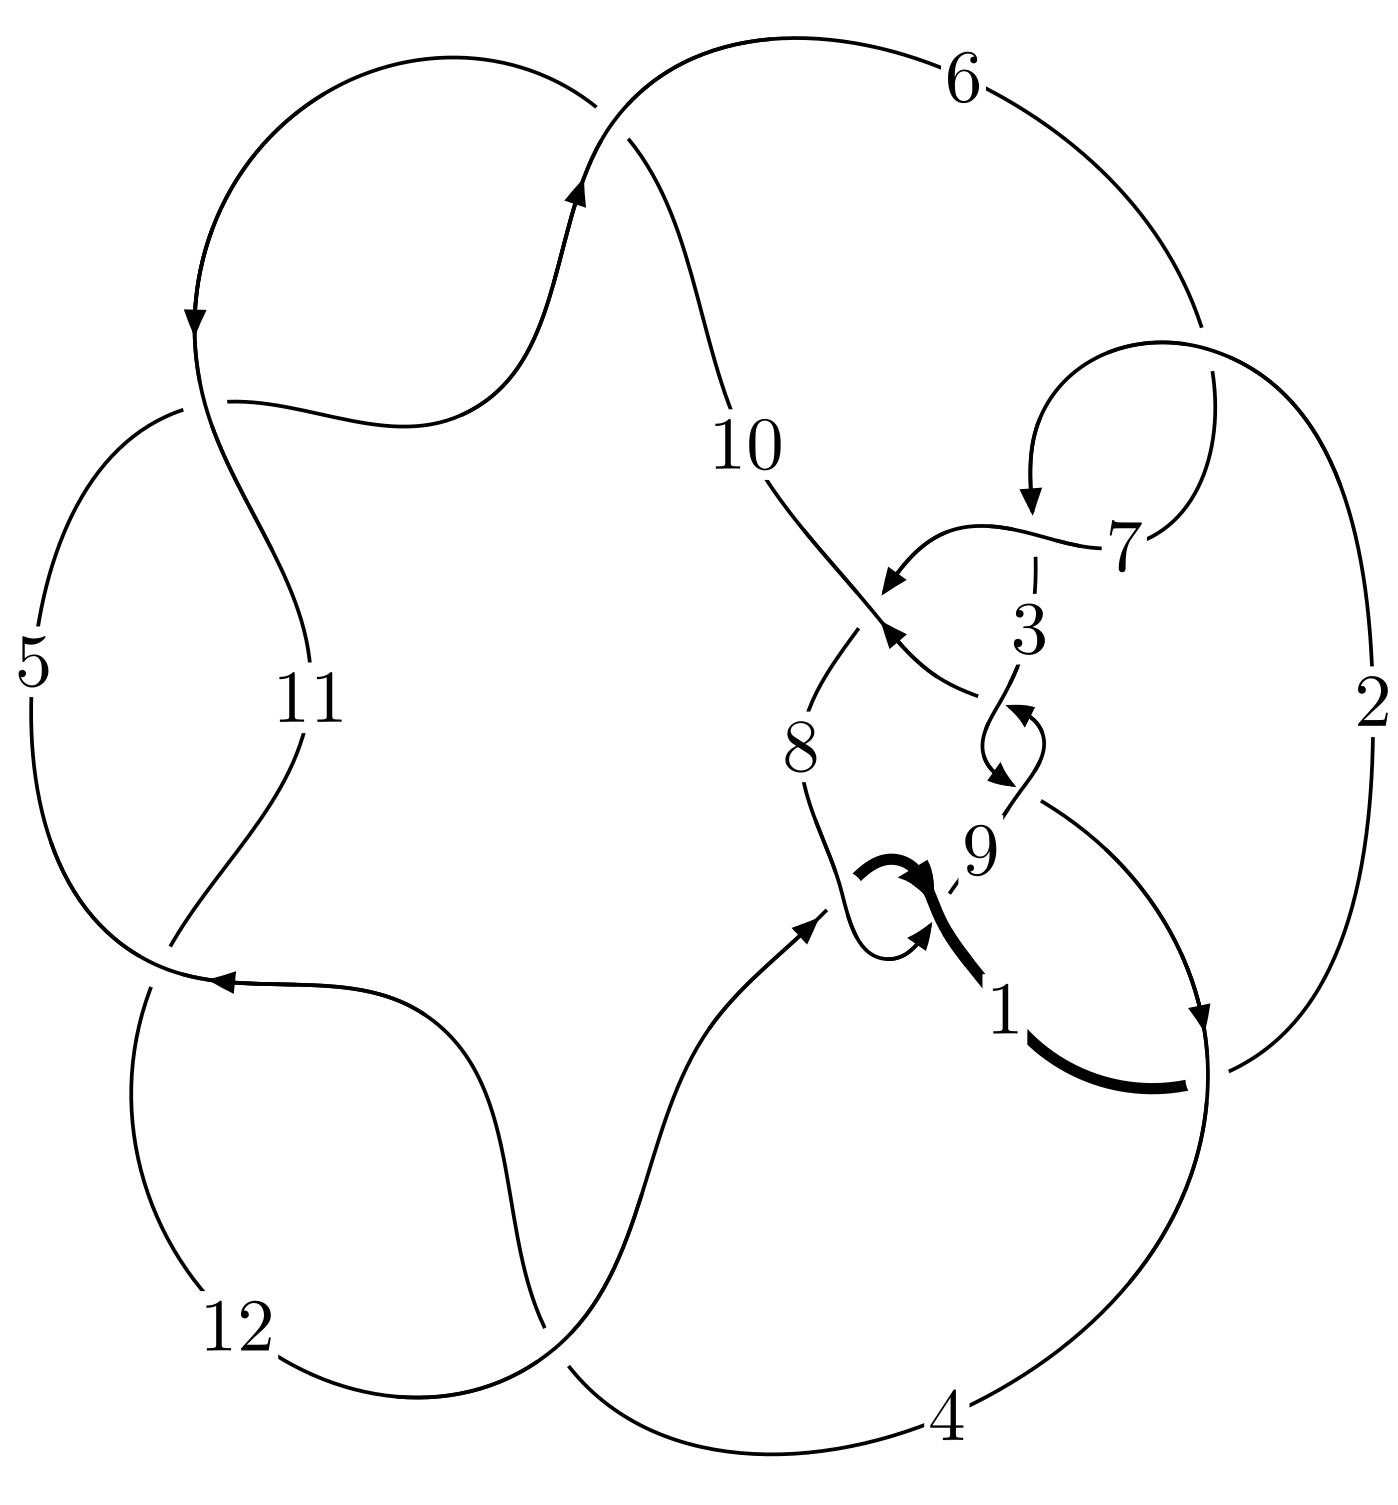
\includegraphics[width=112pt]{../../../GIT/diagram.site/Diagrams/png/1863_12a_1062.png}\\
\ \ \ A knot diagram\footnotemark}&
\allowdisplaybreaks
\textbf{Linearized knot diagam} \\
\cline{2-2}
 &
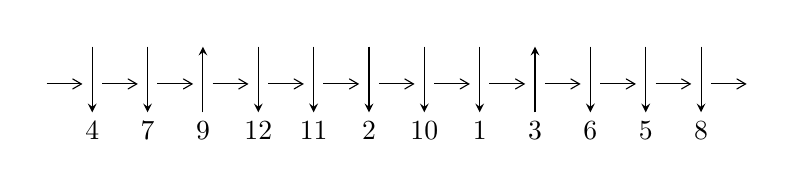
\begin{tikzpicture}[x=20pt, y=17pt]
	% nodes
	\node (C0) at (0, 0) {};
	\node (C1) at (1, 0) {};
	\node (C1U) at (1, +1) {};
	\node (C1D) at (1, -1) {4};

	\node (C2) at (2, 0) {};
	\node (C2U) at (2, +1) {};
	\node (C2D) at (2, -1) {7};

	\node (C3) at (3, 0) {};
	\node (C3U) at (3, +1) {};
	\node (C3D) at (3, -1) {9};

	\node (C4) at (4, 0) {};
	\node (C4U) at (4, +1) {};
	\node (C4D) at (4, -1) {12};

	\node (C5) at (5, 0) {};
	\node (C5U) at (5, +1) {};
	\node (C5D) at (5, -1) {11};

	\node (C6) at (6, 0) {};
	\node (C6U) at (6, +1) {};
	\node (C6D) at (6, -1) {2};

	\node (C7) at (7, 0) {};
	\node (C7U) at (7, +1) {};
	\node (C7D) at (7, -1) {10};

	\node (C8) at (8, 0) {};
	\node (C8U) at (8, +1) {};
	\node (C8D) at (8, -1) {1};

	\node (C9) at (9, 0) {};
	\node (C9U) at (9, +1) {};
	\node (C9D) at (9, -1) {3};

	\node (C10) at (10, 0) {};
	\node (C10U) at (10, +1) {};
	\node (C10D) at (10, -1) {6};

	\node (C11) at (11, 0) {};
	\node (C11U) at (11, +1) {};
	\node (C11D) at (11, -1) {5};

	\node (C12) at (12, 0) {};
	\node (C12U) at (12, +1) {};
	\node (C12D) at (12, -1) {8};
	\node (C13) at (13, 0) {};

	% arrows
	\draw[->,>={angle 60}]
	(C0) edge (C1) (C1) edge (C2) (C2) edge (C3) (C3) edge (C4) (C4) edge (C5) (C5) edge (C6) (C6) edge (C7) (C7) edge (C8) (C8) edge (C9) (C9) edge (C10) (C10) edge (C11) (C11) edge (C12) (C12) edge (C13) ;	\draw[->,>=stealth]
	(C1U) edge (C1D) (C2U) edge (C2D) (C3D) edge (C3U) (C4U) edge (C4D) (C5U) edge (C5D) (C6U) edge (C6D) (C7U) edge (C7D) (C8U) edge (C8D) (C9D) edge (C9U) (C10U) edge (C10D) (C11U) edge (C11D) (C12U) edge (C12D) ;
	\end{tikzpicture} \\
\hhline{~~} \\& 
\textbf{Solving Sequence} \\ \cline{2-2} 
 &
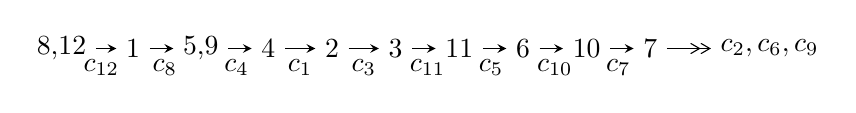
\begin{tikzpicture}[x=23pt, y=7pt]
	% node
	\node (A0) at (-1/8, 0) {8,12};
	\node (A1) at (1, 0) {1};
	\node (A2) at (33/16, 0) {5,9};
	\node (A3) at (25/8, 0) {4};
	\node (A4) at (33/8, 0) {2};
	\node (A5) at (41/8, 0) {3};
	\node (A6) at (49/8, 0) {11};
	\node (A7) at (57/8, 0) {6};
	\node (A8) at (65/8, 0) {10};
	\node (A9) at (73/8, 0) {7};
	\node (C1) at (1/2, -1) {$c_{12}$};
	\node (C2) at (3/2, -1) {$c_{8}$};
	\node (C3) at (21/8, -1) {$c_{4}$};
	\node (C4) at (29/8, -1) {$c_{1}$};
	\node (C5) at (37/8, -1) {$c_{3}$};
	\node (C6) at (45/8, -1) {$c_{11}$};
	\node (C7) at (53/8, -1) {$c_{5}$};
	\node (C8) at (61/8, -1) {$c_{10}$};
	\node (C9) at (69/8, -1) {$c_{7}$};
	\node (A10) at (11, 0) {$c_{2},c_{6},c_{9}$};

	% edge
	\draw[->,>=stealth]	
	(A0) edge (A1) (A1) edge (A2) (A2) edge (A3) (A3) edge (A4) (A4) edge (A5) (A5) edge (A6) (A6) edge (A7) (A7) edge (A8) (A8) edge (A9) ;
	\draw[->>,>={angle 60}]	
	(A9) edge (A10);
\end{tikzpicture} \\ 

\end{tabular} \\

\footnotetext{
The image of knot diagram is generated by the software ``\textbf{Draw programme}" developed by Andrew Bartholomew(\url{http://www.layer8.co.uk/maths/draw/index.htm\#Running-draw}), where we modified some parts for our purpose(\url{https://github.com/CATsTAILs/LinksPainter}).
}\phantom \\ \newline 
\centering \textbf{Ideals for irreducible components\footnotemark of $X_{\text{par}}$} 
 
\begin{align*}
I^u_{1}&=\langle 
-4.35709\times10^{18} u^{28}-2.00758\times10^{18} u^{27}+\cdots+1.77495\times10^{19} b+4.28788\times10^{19},\\
\phantom{I^u_{1}}&\phantom{= \langle  }3.14140\times10^{19} u^{28}-3.48706\times10^{19} u^{27}+\cdots+1.77495\times10^{20} a-6.60203\times10^{19},\;u^{29}- u^{28}+\cdots+6 u+5\rangle \\
I^u_{2}&=\langle 
-6.62139\times10^{45} u^{45}+4.84395\times10^{44} u^{44}+\cdots+2.87295\times10^{46} b+1.78408\times10^{46},\\
\phantom{I^u_{2}}&\phantom{= \langle  }-4.22323\times10^{46} u^{45}+3.37044\times10^{46} u^{44}+\cdots+2.87295\times10^{46} a+3.87573\times10^{46},\;u^{46}- u^{45}+\cdots+72 u^3+1\rangle \\
I^u_{3}&=\langle 
3 b+2 a-1,\;4 a^2+6 a u-4 a-3 u+10,\;u^2+1\rangle \\
I^u_{4}&=\langle 
b,\;a+1,\;u+1\rangle \\
\\
\end{align*}
\raggedright * 4 irreducible components of $\dim_{\mathbb{C}}=0$, with total 80 representations.\\
\footnotetext{All coefficients of polynomials are rational numbers. But the coefficients are sometimes approximated in decimal forms when there is not enough margin.}
\newpage
\renewcommand{\arraystretch}{1}
\centering \section*{I. $I^u_{1}= \langle -4.36\times10^{18} u^{28}-2.01\times10^{18} u^{27}+\cdots+1.77\times10^{19} b+4.29\times10^{19},\;3.14\times10^{19} u^{28}-3.49\times10^{19} u^{27}+\cdots+1.77\times10^{20} a-6.60\times10^{19},\;u^{29}- u^{28}+\cdots+6 u+5 \rangle$}
\flushleft \textbf{(i) Arc colorings}\\
\begin{tabular}{m{7pt} m{180pt} m{7pt} m{180pt} }
\flushright $a_{8}=$&$\begin{pmatrix}0\\u\end{pmatrix}$ \\
\flushright $a_{12}=$&$\begin{pmatrix}1\\0\end{pmatrix}$ \\
\flushright $a_{1}=$&$\begin{pmatrix}1\\u^2\end{pmatrix}$ \\
\flushright $a_{5}=$&$\begin{pmatrix}-0.176986 u^{28}+0.196460 u^{27}+\cdots+4.44222 u+0.371956\\0.245478 u^{28}+0.113107 u^{27}+\cdots-3.74868 u-2.41578\end{pmatrix}$ \\
\flushright $a_{9}=$&$\begin{pmatrix}- u\\- u^3+u\end{pmatrix}$ \\
\flushright $a_{4}=$&$\begin{pmatrix}0.0684919 u^{28}+0.309567 u^{27}+\cdots+0.693541 u-2.04382\\0.245478 u^{28}+0.113107 u^{27}+\cdots-3.74868 u-2.41578\end{pmatrix}$ \\
\flushright $a_{2}=$&$\begin{pmatrix}0.118296 u^{28}-0.0893359 u^{27}+\cdots-3.39351 u+0.162132\\-0.00685004 u^{28}-0.0793457 u^{27}+\cdots-1.42658 u-0.209524\end{pmatrix}$ \\
\flushright $a_{3}=$&$\begin{pmatrix}-0.0781184 u^{28}+0.100703 u^{27}+\cdots+4.05485 u-0.0974079\\0.305018 u^{28}+0.173348 u^{27}+\cdots-4.24410 u-2.58483\end{pmatrix}$ \\
\flushright $a_{11}=$&$\begin{pmatrix}-0.0910595 u^{28}+0.0224573 u^{27}+\cdots+0.754174 u+1.13264\\-0.122205 u^{28}+0.0768161 u^{27}+\cdots+3.17685 u+0.779482\end{pmatrix}$ \\
\flushright $a_{6}=$&$\begin{pmatrix}0.0419048 u^{28}-0.0487548 u^{27}+\cdots-1.40336 u-1.17515\\-0.645066 u^{28}+0.272635 u^{27}+\cdots+6.97049 u+2.35170\end{pmatrix}$ \\
\flushright $a_{10}=$&$\begin{pmatrix}0.105097 u^{28}+0.0315333 u^{27}+\cdots-2.30681 u-0.507286\\-0.0726470 u^{28}+0.0802996 u^{27}+\cdots-2.46182 u-1.60634\end{pmatrix}$ \\
\flushright $a_{7}=$&$\begin{pmatrix}0.0129449 u^{28}-0.0531223 u^{27}+\cdots-0.855717 u-0.583669\\-0.558870 u^{28}+0.260702 u^{27}+\cdots+7.13891 u+2.31745\end{pmatrix}$\\&\end{tabular}
\flushleft \textbf{(ii) Obstruction class $= -1$}\\~\\
\flushleft \textbf{(iii) Cusp Shapes $= \frac{1827767228747590945}{8874731342588739424} u^{28}-\frac{438792885780626433}{4437365671294369712} u^{27}+\cdots-\frac{78225383157899978113}{8874731342588739424} u-\frac{108059866682014660965}{8874731342588739424}$}\\~\\
\newpage\renewcommand{\arraystretch}{1}
\flushleft \textbf{(iv) u-Polynomials at the component}\newline \\
\begin{tabular}{m{50pt}|m{274pt}}
Crossings & \hspace{64pt}u-Polynomials at each crossing \\
\hline $$\begin{aligned}c_{1},c_{7}\end{aligned}$$&$\begin{aligned}
&16(16 u^{29}-48 u^{28}+\cdots+4 u-1)
\end{aligned}$\\
\hline $$\begin{aligned}c_{2},c_{6},c_{8}\\c_{12}\end{aligned}$$&$\begin{aligned}
&u^{29}- u^{28}+\cdots+6 u+5
\end{aligned}$\\
\hline $$\begin{aligned}c_{3},c_{9}\end{aligned}$$&$\begin{aligned}
&u^{29}-3 u^{28}+\cdots-172 u+58
\end{aligned}$\\
\hline $$\begin{aligned}c_{4},c_{5},c_{10}\\c_{11}\end{aligned}$$&$\begin{aligned}
&u^{29}+3 u^{28}+\cdots+68 u+10
\end{aligned}$\\
\hline
\end{tabular}\\~\\
\newpage\renewcommand{\arraystretch}{1}
\flushleft \textbf{(v) Riley Polynomials at the component}\newline \\
\begin{tabular}{m{50pt}|m{274pt}}
Crossings & \hspace{64pt}Riley Polynomials at each crossing \\
\hline $$\begin{aligned}c_{1},c_{7}\end{aligned}$$&$\begin{aligned}
&256(256 y^{29}-640 y^{28}+\cdots+62 y-1)
\end{aligned}$\\
\hline $$\begin{aligned}c_{2},c_{6},c_{8}\\c_{12}\end{aligned}$$&$\begin{aligned}
&y^{29}-11 y^{28}+\cdots+66 y-25
\end{aligned}$\\
\hline $$\begin{aligned}c_{3},c_{9}\end{aligned}$$&$\begin{aligned}
&y^{29}+23 y^{28}+\cdots+9980 y-3364
\end{aligned}$\\
\hline $$\begin{aligned}c_{4},c_{5},c_{10}\\c_{11}\end{aligned}$$&$\begin{aligned}
&y^{29}+33 y^{28}+\cdots-1196 y-100
\end{aligned}$\\
\hline
\end{tabular}\\~\\
\newpage\flushleft \textbf{(vi) Complex Volumes and Cusp Shapes}
$$\begin{array}{c|c|c}  
\text{Solutions to }I^u_{1}& \I (\text{vol} + \sqrt{-1}CS) & \text{Cusp shape}\\
 \hline 
\begin{aligned}
u &= -0.471326 + 0.930518 I \\
a &= -0.32444 - 2.22299 I \\
b &= \phantom{-}0.03883 + 1.63705 I\end{aligned}
 & \phantom{-}11.23150 + 0.31670 I & \phantom{-}0.72463 - 1.97935 I \\ \hline\begin{aligned}
u &= -0.471326 - 0.930518 I \\
a &= -0.32444 + 2.22299 I \\
b &= \phantom{-}0.03883 - 1.63705 I\end{aligned}
 & \phantom{-}11.23150 - 0.31670 I & \phantom{-}0.72463 + 1.97935 I \\ \hline\begin{aligned}
u &= \phantom{-}0.989283 + 0.366561 I \\
a &= -1.123300 + 0.601376 I \\
b &= -0.27077 - 1.51322 I\end{aligned}
 & \phantom{-}3.87255 - 3.92564 I & -7.17073 + 6.57073 I \\ \hline\begin{aligned}
u &= \phantom{-}0.989283 - 0.366561 I \\
a &= -1.123300 - 0.601376 I \\
b &= -0.27077 + 1.51322 I\end{aligned}
 & \phantom{-}3.87255 + 3.92564 I & -7.17073 - 6.57073 I \\ \hline\begin{aligned}
u &= -0.894844 + 0.224932 I \\
a &= \phantom{-}0.609672 + 0.117489 I \\
b &= \phantom{-}0.818306 + 0.515060 I\end{aligned}
 & -2.30220 + 2.09205 I & -7.00937 - 7.58620 I \\ \hline\begin{aligned}
u &= -0.894844 - 0.224932 I \\
a &= \phantom{-}0.609672 - 0.117489 I \\
b &= \phantom{-}0.818306 - 0.515060 I\end{aligned}
 & -2.30220 - 2.09205 I & -7.00937 + 7.58620 I \\ \hline\begin{aligned}
u &= \phantom{-}1.078710 + 0.415737 I \\
a &= \phantom{-}0.868252 - 0.609559 I \\
b &= \phantom{-}0.689515 + 0.698878 I\end{aligned}
 & -1.53035 - 7.20402 I & -9.10388 + 9.44165 I \\ \hline\begin{aligned}
u &= \phantom{-}1.078710 - 0.415737 I \\
a &= \phantom{-}0.868252 + 0.609559 I \\
b &= \phantom{-}0.689515 - 0.698878 I\end{aligned}
 & -1.53035 + 7.20402 I & -9.10388 - 9.44165 I \\ \hline\begin{aligned}
u &= -1.141380 + 0.286143 I \\
a &= -0.164359 + 0.494218 I \\
b &= -0.566117 - 1.168670 I\end{aligned}
 & -5.67885 + 3.21607 I & -12.14399 - 5.43569 I \\ \hline\begin{aligned}
u &= -1.141380 - 0.286143 I \\
a &= -0.164359 - 0.494218 I \\
b &= -0.566117 + 1.168670 I\end{aligned}
 & -5.67885 - 3.21607 I & -12.14399 + 5.43569 I\\
 \hline 
 \end{array}$$\newpage$$\begin{array}{c|c|c}  
\text{Solutions to }I^u_{1}& \I (\text{vol} + \sqrt{-1}CS) & \text{Cusp shape}\\
 \hline 
\begin{aligned}
u &= \phantom{-}0.422423 + 0.698933 I \\
a &= -0.308566 + 0.892792 I \\
b &= \phantom{-}0.101826 - 0.815142 I\end{aligned}
 & \phantom{-}2.73932 - 0.92739 I & \phantom{-}0.75660 + 2.98272 I \\ \hline\begin{aligned}
u &= \phantom{-}0.422423 - 0.698933 I \\
a &= -0.308566 - 0.892792 I \\
b &= \phantom{-}0.101826 + 0.815142 I\end{aligned}
 & \phantom{-}2.73932 + 0.92739 I & \phantom{-}0.75660 - 2.98272 I \\ \hline\begin{aligned}
u &= \phantom{-}0.746623 + 0.193942 I \\
a &= \phantom{-}0.902000 - 0.966773 I \\
b &= \phantom{-}0.06012 + 1.74114 I\end{aligned}
 & \phantom{-}6.12616 - 1.21646 I & -4.32561 + 4.57305 I \\ \hline\begin{aligned}
u &= \phantom{-}0.746623 - 0.193942 I \\
a &= \phantom{-}0.902000 + 0.966773 I \\
b &= \phantom{-}0.06012 - 1.74114 I\end{aligned}
 & \phantom{-}6.12616 + 1.21646 I & -4.32561 - 4.57305 I \\ \hline\begin{aligned}
u &= -0.746883\phantom{ +0.000000I} \\
a &= -0.860796\phantom{ +0.000000I} \\
b &= -0.796318\phantom{ +0.000000I}\end{aligned}
 & -1.46174\phantom{ +0.000000I} & -3.54150\phantom{ +0.000000I} \\ \hline\begin{aligned}
u &= -0.236709 + 1.286190 I \\
a &= \phantom{-}0.060143 + 0.822295 I \\
b &= -0.237684 - 0.540453 I\end{aligned}
 & \phantom{-}0.525909 - 0.884260 I & -11.9177 + 8.2327 I \\ \hline\begin{aligned}
u &= -0.236709 - 1.286190 I \\
a &= \phantom{-}0.060143 - 0.822295 I \\
b &= -0.237684 + 0.540453 I\end{aligned}
 & \phantom{-}0.525909 + 0.884260 I & -11.9177 - 8.2327 I \\ \hline\begin{aligned}
u &= -1.186580 + 0.554420 I \\
a &= \phantom{-}1.39175 + 1.13943 I \\
b &= \phantom{-}0.20443 - 1.61493 I\end{aligned}
 & \phantom{-}6.24626 + 10.51930 I & -6.12287 - 7.23991 I \\ \hline\begin{aligned}
u &= -1.186580 - 0.554420 I \\
a &= \phantom{-}1.39175 - 1.13943 I \\
b &= \phantom{-}0.20443 + 1.61493 I\end{aligned}
 & \phantom{-}6.24626 - 10.51930 I & -6.12287 + 7.23991 I \\ \hline\begin{aligned}
u &= \phantom{-}1.278090 + 0.410634 I \\
a &= -0.327813 + 0.182357 I \\
b &= -0.845051 + 0.136443 I\end{aligned}
 & -9.57615 - 8.03561 I & -14.4420 + 5.3510 I\\
 \hline 
 \end{array}$$\newpage$$\begin{array}{c|c|c}  
\text{Solutions to }I^u_{1}& \I (\text{vol} + \sqrt{-1}CS) & \text{Cusp shape}\\
 \hline 
\begin{aligned}
u &= \phantom{-}1.278090 - 0.410634 I \\
a &= -0.327813 - 0.182357 I \\
b &= -0.845051 - 0.136443 I\end{aligned}
 & -9.57615 + 8.03561 I & -14.4420 - 5.3510 I \\ \hline\begin{aligned}
u &= -1.32626 + 0.52915 I \\
a &= -0.750008 - 0.859966 I \\
b &= -0.629916 + 0.818379 I\end{aligned}
 & -7.5127 + 12.8935 I & -11.3843 - 8.7195 I \\ \hline\begin{aligned}
u &= -1.32626 - 0.52915 I \\
a &= -0.750008 + 0.859966 I \\
b &= -0.629916 - 0.818379 I\end{aligned}
 & -7.5127 - 12.8935 I & -11.3843 + 8.7195 I \\ \hline\begin{aligned}
u &= \phantom{-}1.34660 + 0.62954 I \\
a &= -1.33868 + 1.46318 I \\
b &= -0.19137 - 1.64914 I\end{aligned}
 & \phantom{-}0.8405 - 16.0516 I & -8.77423 + 7.86114 I \\ \hline\begin{aligned}
u &= \phantom{-}1.34660 - 0.62954 I \\
a &= -1.33868 - 1.46318 I \\
b &= -0.19137 + 1.64914 I\end{aligned}
 & \phantom{-}0.8405 + 16.0516 I & -8.77423 - 7.86114 I \\ \hline\begin{aligned}
u &= \phantom{-}0.46363 + 1.46562 I \\
a &= \phantom{-}0.07882 - 2.15458 I \\
b &= -0.06154 + 1.57781 I\end{aligned}
 & \phantom{-}7.86481 + 1.93517 I & -8.22751 - 3.59914 I \\ \hline\begin{aligned}
u &= \phantom{-}0.46363 - 1.46562 I \\
a &= \phantom{-}0.07882 + 2.15458 I \\
b &= -0.06154 - 1.57781 I\end{aligned}
 & \phantom{-}7.86481 - 1.93517 I & -8.22751 + 3.59914 I \\ \hline\begin{aligned}
u &= -0.194808 + 0.345152 I \\
a &= -0.943074 + 0.687123 I \\
b &= -0.212425 + 0.288508 I\end{aligned}
 & -0.601308 + 0.869978 I & -10.08823 - 7.77060 I \\ \hline\begin{aligned}
u &= -0.194808 - 0.345152 I \\
a &= -0.943074 - 0.687123 I \\
b &= -0.212425 - 0.288508 I\end{aligned}
 & -0.601308 - 0.869978 I & -10.08823 + 7.77060 I\\
 \hline 
 \end{array}$$\newpage\newpage\renewcommand{\arraystretch}{1}
\centering \section*{II. $I^u_{2}= \langle -6.62\times10^{45} u^{45}+4.84\times10^{44} u^{44}+\cdots+2.87\times10^{46} b+1.78\times10^{46},\;-4.22\times10^{46} u^{45}+3.37\times10^{46} u^{44}+\cdots+2.87\times10^{46} a+3.88\times10^{46},\;u^{46}- u^{45}+\cdots+72 u^3+1 \rangle$}
\flushleft \textbf{(i) Arc colorings}\\
\begin{tabular}{m{7pt} m{180pt} m{7pt} m{180pt} }
\flushright $a_{8}=$&$\begin{pmatrix}0\\u\end{pmatrix}$ \\
\flushright $a_{12}=$&$\begin{pmatrix}1\\0\end{pmatrix}$ \\
\flushright $a_{1}=$&$\begin{pmatrix}1\\u^2\end{pmatrix}$ \\
\flushright $a_{5}=$&$\begin{pmatrix}1.47000 u^{45}-1.17316 u^{44}+\cdots+20.0764 u-1.34904\\0.230474 u^{45}-0.0168606 u^{44}+\cdots-1.54825 u-0.620995\end{pmatrix}$ \\
\flushright $a_{9}=$&$\begin{pmatrix}- u\\- u^3+u\end{pmatrix}$ \\
\flushright $a_{4}=$&$\begin{pmatrix}1.70047 u^{45}-1.19003 u^{44}+\cdots+18.5281 u-1.97004\\0.230474 u^{45}-0.0168606 u^{44}+\cdots-1.54825 u-0.620995\end{pmatrix}$ \\
\flushright $a_{2}=$&$\begin{pmatrix}0.185550 u^{45}-0.0904179 u^{44}+\cdots+13.6824 u+6.31036\\0.00565620 u^{45}-0.104925 u^{44}+\cdots+1.19083 u+0.432576\end{pmatrix}$ \\
\flushright $a_{3}=$&$\begin{pmatrix}1.51125 u^{45}-1.22829 u^{44}+\cdots+20.2705 u-1.45837\\0.0893100 u^{45}+0.110629 u^{44}+\cdots-3.10135 u-0.905173\end{pmatrix}$ \\
\flushright $a_{11}=$&$\begin{pmatrix}-0.456685 u^{45}-0.420359 u^{44}+\cdots-9.08457 u-4.32491\\-0.583337 u^{45}+0.373887 u^{44}+\cdots-0.150803 u+0.653918\end{pmatrix}$ \\
\flushright $a_{6}=$&$\begin{pmatrix}0.151527 u^{45}+0.286238 u^{44}+\cdots+8.26354 u+0.627866\\-0.825790 u^{45}+0.358853 u^{44}+\cdots+3.50116 u+2.03572\end{pmatrix}$ \\
\flushright $a_{10}=$&$\begin{pmatrix}0.521385 u^{45}-0.153313 u^{44}+\cdots+0.495270 u-4.38356\\1.05862 u^{45}-0.639836 u^{44}+\cdots+5.19161 u-1.11148\end{pmatrix}$ \\
\flushright $a_{7}=$&$\begin{pmatrix}0.840952 u^{45}-0.757829 u^{44}+\cdots+18.1621 u+2.90992\\-1.32879 u^{45}+0.828964 u^{44}+\cdots-2.95845 u+2.16499\end{pmatrix}$\\&\end{tabular}
\flushleft \textbf{(ii) Obstruction class $= -1$}\\~\\
\flushleft \textbf{(iii) Cusp Shapes $= -2.26393 u^{45}+0.703208 u^{44}+\cdots+0.508567 u-4.58033$}\\~\\
\newpage\renewcommand{\arraystretch}{1}
\flushleft \textbf{(iv) u-Polynomials at the component}\newline \\
\begin{tabular}{m{50pt}|m{274pt}}
Crossings & \hspace{64pt}u-Polynomials at each crossing \\
\hline $$\begin{aligned}c_{1},c_{7}\end{aligned}$$&$\begin{aligned}
&25(25 u^{46}+105 u^{45}+\cdots+114436 u-17519)
\end{aligned}$\\
\hline $$\begin{aligned}c_{2},c_{6},c_{8}\\c_{12}\end{aligned}$$&$\begin{aligned}
&u^{46}- u^{45}+\cdots+72 u^3+1
\end{aligned}$\\
\hline $$\begin{aligned}c_{3},c_{9}\end{aligned}$$&$\begin{aligned}
&(u^{23}+u^{22}+\cdots+2 u+1)^{2}
\end{aligned}$\\
\hline $$\begin{aligned}c_{4},c_{5},c_{10}\\c_{11}\end{aligned}$$&$\begin{aligned}
&(u^{23}- u^{22}+\cdots-2 u+1)^{2}
\end{aligned}$\\
\hline
\end{tabular}\\~\\
\newpage\renewcommand{\arraystretch}{1}
\flushleft \textbf{(v) Riley Polynomials at the component}\newline \\
\begin{tabular}{m{50pt}|m{274pt}}
Crossings & \hspace{64pt}Riley Polynomials at each crossing \\
\hline $$\begin{aligned}c_{1},c_{7}\end{aligned}$$&$\begin{aligned}
&625(625 y^{46}-13125 y^{45}+\cdots-2.98321\times10^{9} y+3.06915\times10^{8})
\end{aligned}$\\
\hline $$\begin{aligned}c_{2},c_{6},c_{8}\\c_{12}\end{aligned}$$&$\begin{aligned}
&y^{46}-29 y^{45}+\cdots-364 y^2+1
\end{aligned}$\\
\hline $$\begin{aligned}c_{3},c_{9}\end{aligned}$$&$\begin{aligned}
&(y^{23}+19 y^{22}+\cdots-4 y-1)^{2}
\end{aligned}$\\
\hline $$\begin{aligned}c_{4},c_{5},c_{10}\\c_{11}\end{aligned}$$&$\begin{aligned}
&(y^{23}+27 y^{22}+\cdots-4 y-1)^{2}
\end{aligned}$\\
\hline
\end{tabular}\\~\\
\newpage\flushleft \textbf{(vi) Complex Volumes and Cusp Shapes}
$$\begin{array}{c|c|c}  
\text{Solutions to }I^u_{2}& \I (\text{vol} + \sqrt{-1}CS) & \text{Cusp shape}\\
 \hline 
\begin{aligned}
u &= \phantom{-}0.960668 + 0.217642 I \\
a &= \phantom{-}1.60344 - 1.21245 I \\
b &= \phantom{-}0.228067 + 0.467269 I\end{aligned}
 & -3.14970 - 0.92592 I & -9.05751 + 7.44214 I \\ \hline\begin{aligned}
u &= \phantom{-}0.960668 - 0.217642 I \\
a &= \phantom{-}1.60344 + 1.21245 I \\
b &= \phantom{-}0.228067 - 0.467269 I\end{aligned}
 & -3.14970 + 0.92592 I & -9.05751 - 7.44214 I \\ \hline\begin{aligned}
u &= \phantom{-}0.944170 + 0.194325 I \\
a &= \phantom{-}1.66541 - 0.85193 I \\
b &= \phantom{-}0.09185 + 1.62814 I\end{aligned}
 & \phantom{-}5.85259 - 0.83337 I & -5.37353 - 0.43888 I \\ \hline\begin{aligned}
u &= \phantom{-}0.944170 - 0.194325 I \\
a &= \phantom{-}1.66541 + 0.85193 I \\
b &= \phantom{-}0.09185 - 1.62814 I\end{aligned}
 & \phantom{-}5.85259 + 0.83337 I & -5.37353 + 0.43888 I \\ \hline\begin{aligned}
u &= -0.260832 + 0.901044 I \\
a &= \phantom{-}0.10902 + 2.08680 I \\
b &= -0.11785 - 1.62483 I\end{aligned}
 & \phantom{-}9.09029 - 5.22748 I & -2.33369 + 3.33432 I \\ \hline\begin{aligned}
u &= -0.260832 - 0.901044 I \\
a &= \phantom{-}0.10902 - 2.08680 I \\
b &= -0.11785 + 1.62483 I\end{aligned}
 & \phantom{-}9.09029 + 5.22748 I & -2.33369 - 3.33432 I \\ \hline\begin{aligned}
u &= -1.060680 + 0.129047 I \\
a &= \phantom{-}0.965371 - 0.700301 I \\
b &= \phantom{-}0.324148 + 0.802707 I\end{aligned}
 & -2.47271 + 0.74531 I & -6.91991 + 0.73522 I \\ \hline\begin{aligned}
u &= -1.060680 - 0.129047 I \\
a &= \phantom{-}0.965371 + 0.700301 I \\
b &= \phantom{-}0.324148 - 0.802707 I\end{aligned}
 & -2.47271 - 0.74531 I & -6.91991 - 0.73522 I \\ \hline\begin{aligned}
u &= -0.978562 + 0.439060 I \\
a &= \phantom{-}2.30652 + 1.97958 I \\
b &= \phantom{-}0.03322 - 1.55779 I\end{aligned}
 & \phantom{-}3.82738 + 1.68405 I & -5.64484 - 3.83025 I \\ \hline\begin{aligned}
u &= -0.978562 - 0.439060 I \\
a &= \phantom{-}2.30652 - 1.97958 I \\
b &= \phantom{-}0.03322 + 1.55779 I\end{aligned}
 & \phantom{-}3.82738 - 1.68405 I & -5.64484 + 3.83025 I\\
 \hline 
 \end{array}$$\newpage$$\begin{array}{c|c|c}  
\text{Solutions to }I^u_{2}& \I (\text{vol} + \sqrt{-1}CS) & \text{Cusp shape}\\
 \hline 
\begin{aligned}
u &= -0.032046 + 1.078310 I \\
a &= -0.130214 - 0.963704 I \\
b &= \phantom{-}0.473302 + 0.738923 I\end{aligned}
 & -3.45327 - 7.25342 I & -8.90266 + 7.25802 I \\ \hline\begin{aligned}
u &= -0.032046 - 1.078310 I \\
a &= -0.130214 + 0.963704 I \\
b &= \phantom{-}0.473302 - 0.738923 I\end{aligned}
 & -3.45327 + 7.25342 I & -8.90266 - 7.25802 I \\ \hline\begin{aligned}
u &= \phantom{-}1.013490 + 0.406902 I \\
a &= -0.920257 + 0.717264 I \\
b &= -0.413689 - 0.761868 I\end{aligned}
 & \phantom{-}0.92198 - 3.22031 I & -3.77921 + 4.90443 I \\ \hline\begin{aligned}
u &= \phantom{-}1.013490 - 0.406902 I \\
a &= -0.920257 - 0.717264 I \\
b &= -0.413689 + 0.761868 I\end{aligned}
 & \phantom{-}0.92198 + 3.22031 I & -3.77921 - 4.90443 I \\ \hline\begin{aligned}
u &= -0.882714\phantom{ +0.000000I} \\
a &= -0.656431\phantom{ +0.000000I} \\
b &= -0.546774\phantom{ +0.000000I}\end{aligned}
 & -1.28214\phantom{ +0.000000I} & -7.98830\phantom{ +0.000000I} \\ \hline\begin{aligned}
u &= -1.116100 + 0.137828 I \\
a &= \phantom{-}0.095732 + 0.799884 I \\
b &= \phantom{-}0.228067 + 0.467269 I\end{aligned}
 & -3.14970 - 0.92592 I & -9.05751 + 7.44214 I \\ \hline\begin{aligned}
u &= -1.116100 - 0.137828 I \\
a &= \phantom{-}0.095732 - 0.799884 I \\
b &= \phantom{-}0.228067 - 0.467269 I\end{aligned}
 & -3.14970 + 0.92592 I & -9.05751 - 7.44214 I \\ \hline\begin{aligned}
u &= -0.151468 + 0.832504 I \\
a &= -0.148349 - 0.609597 I \\
b &= \phantom{-}0.581337 + 0.108709 I\end{aligned}
 & -5.29586 + 3.66457 I & -12.82434 - 2.67133 I \\ \hline\begin{aligned}
u &= -0.151468 - 0.832504 I \\
a &= -0.148349 + 0.609597 I \\
b &= \phantom{-}0.581337 - 0.108709 I\end{aligned}
 & -5.29586 - 3.66457 I & -12.82434 + 2.67133 I \\ \hline\begin{aligned}
u &= \phantom{-}0.174340 + 1.236240 I \\
a &= \phantom{-}0.13883 + 2.25785 I \\
b &= \phantom{-}0.13674 - 1.61894 I\end{aligned}
 & \phantom{-}4.58136 + 9.54664 I & -8.00000 - 5.57899 I\\
 \hline 
 \end{array}$$\newpage$$\begin{array}{c|c|c}  
\text{Solutions to }I^u_{2}& \I (\text{vol} + \sqrt{-1}CS) & \text{Cusp shape}\\
 \hline 
\begin{aligned}
u &= \phantom{-}0.174340 - 1.236240 I \\
a &= \phantom{-}0.13883 - 2.25785 I \\
b &= \phantom{-}0.13674 + 1.61894 I\end{aligned}
 & \phantom{-}4.58136 - 9.54664 I & -8.00000 + 5.57899 I \\ \hline\begin{aligned}
u &= -1.125600 + 0.590859 I \\
a &= -1.39957 - 1.39854 I \\
b &= -0.11785 + 1.62483 I\end{aligned}
 & \phantom{-}9.09029 + 5.22748 I & \phantom{-0.000000 } 0 \\ \hline\begin{aligned}
u &= -1.125600 - 0.590859 I \\
a &= -1.39957 + 1.39854 I \\
b &= -0.11785 - 1.62483 I\end{aligned}
 & \phantom{-}9.09029 - 5.22748 I & \phantom{-0.000000 } 0 \\ \hline\begin{aligned}
u &= \phantom{-}1.263600 + 0.196622 I \\
a &= -0.723405 - 0.104554 I \\
b &= \phantom{-}0.03322 - 1.55779 I\end{aligned}
 & \phantom{-}3.82738 + 1.68405 I & -8.00000 - 3.83025 I \\ \hline\begin{aligned}
u &= \phantom{-}1.263600 - 0.196622 I \\
a &= -0.723405 + 0.104554 I \\
b &= \phantom{-}0.03322 + 1.55779 I\end{aligned}
 & \phantom{-}3.82738 - 1.68405 I & -8.00000 + 3.83025 I \\ \hline\begin{aligned}
u &= \phantom{-}0.223468 + 0.627017 I \\
a &= \phantom{-}0.304838 - 0.560630 I \\
b &= -0.413689 + 0.761868 I\end{aligned}
 & \phantom{-}0.92198 + 3.22031 I & -3.77921 - 4.90443 I \\ \hline\begin{aligned}
u &= \phantom{-}0.223468 - 0.627017 I \\
a &= \phantom{-}0.304838 + 0.560630 I \\
b &= -0.413689 - 0.761868 I\end{aligned}
 & \phantom{-}0.92198 - 3.22031 I & -3.77921 + 4.90443 I \\ \hline\begin{aligned}
u &= \phantom{-}1.303950 + 0.339252 I \\
a &= \phantom{-}0.418446 + 0.083716 I \\
b &= \phantom{-}0.581337 - 0.108709 I\end{aligned}
 & -5.29586 - 3.66457 I & \phantom{-0.000000 } 0 \\ \hline\begin{aligned}
u &= \phantom{-}1.303950 - 0.339252 I \\
a &= \phantom{-}0.418446 - 0.083716 I \\
b &= \phantom{-}0.581337 + 0.108709 I\end{aligned}
 & -5.29586 + 3.66457 I & \phantom{-0.000000 } 0 \\ \hline\begin{aligned}
u &= -1.250840 + 0.612691 I \\
a &= -0.441738 - 0.907872 I \\
b &= -0.477903 + 0.451361 I\end{aligned}
 & -8.25826 + 1.68040 I & \phantom{-0.000000 } 0\\
 \hline 
 \end{array}$$\newpage$$\begin{array}{c|c|c}  
\text{Solutions to }I^u_{2}& \I (\text{vol} + \sqrt{-1}CS) & \text{Cusp shape}\\
 \hline 
\begin{aligned}
u &= -1.250840 - 0.612691 I \\
a &= -0.441738 + 0.907872 I \\
b &= -0.477903 - 0.451361 I\end{aligned}
 & -8.25826 - 1.68040 I & \phantom{-0.000000 } 0 \\ \hline\begin{aligned}
u &= \phantom{-}1.09538 + 0.90096 I \\
a &= -0.88861 + 2.13172 I \\
b &= -0.08584 - 1.50808 I\end{aligned}
 & -1.82520 - 3.53591 I & \phantom{-0.000000 } 0 \\ \hline\begin{aligned}
u &= \phantom{-}1.09538 - 0.90096 I \\
a &= -0.88861 - 2.13172 I \\
b &= -0.08584 + 1.50808 I\end{aligned}
 & -1.82520 + 3.53591 I & \phantom{-0.000000 } 0 \\ \hline\begin{aligned}
u &= -1.35206 + 0.55810 I \\
a &= \phantom{-}0.633793 + 0.759928 I \\
b &= \phantom{-}0.473302 - 0.738923 I\end{aligned}
 & -3.45327 + 7.25342 I & \phantom{-0.000000 } 0 \\ \hline\begin{aligned}
u &= -1.35206 - 0.55810 I \\
a &= \phantom{-}0.633793 - 0.759928 I \\
b &= \phantom{-}0.473302 + 0.738923 I\end{aligned}
 & -3.45327 - 7.25342 I & \phantom{-0.000000 } 0 \\ \hline\begin{aligned}
u &= \phantom{-}1.42000 + 0.41703 I \\
a &= -0.051313 - 0.188624 I \\
b &= -0.477903 + 0.451361 I\end{aligned}
 & -8.25826 + 1.68040 I & \phantom{-0.000000 } 0 \\ \hline\begin{aligned}
u &= \phantom{-}1.42000 - 0.41703 I \\
a &= -0.051313 + 0.188624 I \\
b &= -0.477903 - 0.451361 I\end{aligned}
 & -8.25826 - 1.68040 I & \phantom{-0.000000 } 0 \\ \hline\begin{aligned}
u &= \phantom{-}1.37422 + 0.72873 I \\
a &= \phantom{-}1.09577 - 1.56402 I \\
b &= \phantom{-}0.13674 + 1.61894 I\end{aligned}
 & \phantom{-}4.58136 - 9.54664 I & \phantom{-0.000000 } 0 \\ \hline\begin{aligned}
u &= \phantom{-}1.37422 - 0.72873 I \\
a &= \phantom{-}1.09577 + 1.56402 I \\
b &= \phantom{-}0.13674 - 1.61894 I\end{aligned}
 & \phantom{-}4.58136 + 9.54664 I & \phantom{-0.000000 } 0 \\ \hline\begin{aligned}
u &= \phantom{-}0.165356 + 0.313036 I \\
a &= -2.30752 + 0.60796 I \\
b &= \phantom{-}0.09185 - 1.62814 I\end{aligned}
 & \phantom{-}5.85259 + 0.83337 I & -5.37353 + 0.43888 I\\
 \hline 
 \end{array}$$\newpage$$\begin{array}{c|c|c}  
\text{Solutions to }I^u_{2}& \I (\text{vol} + \sqrt{-1}CS) & \text{Cusp shape}\\
 \hline 
\begin{aligned}
u &= \phantom{-}0.165356 - 0.313036 I \\
a &= -2.30752 - 0.60796 I \\
b &= \phantom{-}0.09185 + 1.62814 I\end{aligned}
 & \phantom{-}5.85259 - 0.83337 I & -5.37353 - 0.43888 I \\ \hline\begin{aligned}
u &= -1.63171 + 0.23232 I \\
a &= \phantom{-}0.114074 + 1.088240 I \\
b &= -0.08584 - 1.50808 I\end{aligned}
 & -1.82520 - 3.53591 I & \phantom{-0.000000 } 0 \\ \hline\begin{aligned}
u &= -1.63171 - 0.23232 I \\
a &= \phantom{-}0.114074 - 1.088240 I \\
b &= -0.08584 + 1.50808 I\end{aligned}
 & -1.82520 + 3.53591 I & \phantom{-0.000000 } 0 \\ \hline\begin{aligned}
u &= \phantom{-}0.064261 + 0.284784 I \\
a &= \phantom{-}2.76905 + 3.46178 I \\
b &= \phantom{-}0.324148 - 0.802707 I\end{aligned}
 & -2.47271 - 0.74531 I & -6.91991 - 0.73522 I \\ \hline\begin{aligned}
u &= \phantom{-}0.064261 - 0.284784 I \\
a &= \phantom{-}2.76905 - 3.46178 I \\
b &= \phantom{-}0.324148 + 0.802707 I\end{aligned}
 & -2.47271 + 0.74531 I & -6.91991 + 0.73522 I \\ \hline\begin{aligned}
u &= -0.203324\phantom{ +0.000000I} \\
a &= -2.56222\phantom{ +0.000000I} \\
b &= -0.546774\phantom{ +0.000000I}\end{aligned}
 & -1.28214\phantom{ +0.000000I} & -7.98830\phantom{ +0.000000I}\\
 \hline 
 \end{array}$$\newpage\newpage\renewcommand{\arraystretch}{1}
\centering \section*{III. $I^u_{3}= \langle 3 b+2 a-1,\;4 a^2+6 a u-4 a-3 u+10,\;u^2+1 \rangle$}
\flushleft \textbf{(i) Arc colorings}\\
\begin{tabular}{m{7pt} m{180pt} m{7pt} m{180pt} }
\flushright $a_{8}=$&$\begin{pmatrix}0\\u\end{pmatrix}$ \\
\flushright $a_{12}=$&$\begin{pmatrix}1\\0\end{pmatrix}$ \\
\flushright $a_{1}=$&$\begin{pmatrix}1\\-1\end{pmatrix}$ \\
\flushright $a_{5}=$&$\begin{pmatrix}a\\-\frac{2}{3} a+\frac{1}{3}\end{pmatrix}$ \\
\flushright $a_{9}=$&$\begin{pmatrix}- u\\2 u\end{pmatrix}$ \\
\flushright $a_{4}=$&$\begin{pmatrix}\frac{1}{3} a+\frac{1}{3}\\-\frac{2}{3} a+\frac{1}{3}\end{pmatrix}$ \\
\flushright $a_{2}=$&$\begin{pmatrix}\frac{1}{6} a u-\frac{1}{12} u+\frac{3}{2}\\-\frac{1}{3} a u-\frac{1}{3} a+\frac{1}{6} u-\frac{4}{3}\end{pmatrix}$ \\
\flushright $a_{3}=$&$\begin{pmatrix}\frac{1}{3} a+\frac{4}{3}\\-\frac{2}{3} a-\frac{5}{3}\end{pmatrix}$ \\
\flushright $a_{11}=$&$\begin{pmatrix}- a u+\frac{1}{3} a+\frac{1}{2} u-\frac{2}{3}\\\frac{2}{3} a u-\frac{1}{3} u+1\end{pmatrix}$ \\
\flushright $a_{6}=$&$\begin{pmatrix}-\frac{1}{3} a u-\frac{1}{3} a+\frac{5}{3} u+\frac{1}{6}\\\frac{2}{3} a- u-\frac{1}{3}\end{pmatrix}$ \\
\flushright $a_{10}=$&$\begin{pmatrix}\frac{1}{3} a u+\frac{1}{3} u\\-\frac{2}{3} a u+\frac{1}{3} u\end{pmatrix}$ \\
\flushright $a_{7}=$&$\begin{pmatrix}-\frac{1}{3} a u-\frac{1}{6} a+\frac{1}{6} u+\frac{1}{12}\\\frac{1}{3} a u+\frac{1}{3} a+\frac{1}{3} u-\frac{1}{6}\end{pmatrix}$\\&\end{tabular}
\flushleft \textbf{(ii) Obstruction class $= 1$}\\~\\
\flushleft \textbf{(iii) Cusp Shapes $= -4$}\\~\\
\newpage\renewcommand{\arraystretch}{1}
\flushleft \textbf{(iv) u-Polynomials at the component}\newline \\
\begin{tabular}{m{50pt}|m{274pt}}
Crossings & \hspace{64pt}u-Polynomials at each crossing \\
\hline $$\begin{aligned}c_{1},c_{7}\end{aligned}$$&$\begin{aligned}
&16(16 u^4-32 u^3+36 u^2-20 u+5)
\end{aligned}$\\
\hline $$\begin{aligned}c_{2},c_{3},c_{6}\\c_{8},c_{9},c_{12}\end{aligned}$$&$\begin{aligned}
&(u^2+1)^2
\end{aligned}$\\
\hline $$\begin{aligned}c_{4},c_{5},c_{10}\\c_{11}\end{aligned}$$&$\begin{aligned}
&u^4+3 u^2+1
\end{aligned}$\\
\hline
\end{tabular}\\~\\
\newpage\renewcommand{\arraystretch}{1}
\flushleft \textbf{(v) Riley Polynomials at the component}\newline \\
\begin{tabular}{m{50pt}|m{274pt}}
Crossings & \hspace{64pt}Riley Polynomials at each crossing \\
\hline $$\begin{aligned}c_{1},c_{7}\end{aligned}$$&$\begin{aligned}
&256(256 y^4+128 y^3+176 y^2-40 y+25)
\end{aligned}$\\
\hline $$\begin{aligned}c_{2},c_{3},c_{6}\\c_{8},c_{9},c_{12}\end{aligned}$$&$\begin{aligned}
&(y+1)^4
\end{aligned}$\\
\hline $$\begin{aligned}c_{4},c_{5},c_{10}\\c_{11}\end{aligned}$$&$\begin{aligned}
&(y^2+3 y+1)^2
\end{aligned}$\\
\hline
\end{tabular}\\~\\
\newpage\flushleft \textbf{(vi) Complex Volumes and Cusp Shapes}
$$\begin{array}{c|c|c}  
\text{Solutions to }I^u_{3}& \I (\text{vol} + \sqrt{-1}CS) & \text{Cusp shape}\\
 \hline 
\begin{aligned}
u &= \phantom{-0.000000 -}1.000000 I \\
a &= \phantom{-}0.500000 + 0.927051 I \\
b &= \phantom{-0.000000 } -0.618034 I\end{aligned}
 & \phantom{-}0.986960\phantom{ +0.000000I} & -4.00000\phantom{ +0.000000I} \\ \hline\begin{aligned}
u &= \phantom{-0.000000 -}1.000000 I \\
a &= \phantom{-}0.50000 - 2.42705 I \\
b &= \phantom{-0.000000 -}1.61803 I\end{aligned}
 & \phantom{-}8.88264\phantom{ +0.000000I} & -4.00000\phantom{ +0.000000I} \\ \hline\begin{aligned}
u &= \phantom{-0.000000 } -1.000000 I \\
a &= \phantom{-}0.500000 - 0.927051 I \\
b &= \phantom{-0.000000 -}0.618034 I\end{aligned}
 & \phantom{-}0.986960\phantom{ +0.000000I} & -4.00000\phantom{ +0.000000I} \\ \hline\begin{aligned}
u &= \phantom{-0.000000 } -1.000000 I \\
a &= \phantom{-}0.50000 + 2.42705 I \\
b &= \phantom{-0.000000 } -1.61803 I\end{aligned}
 & \phantom{-}8.88264\phantom{ +0.000000I} & -4.00000\phantom{ +0.000000I}\\
 \hline 
 \end{array}$$\newpage\newpage\renewcommand{\arraystretch}{1}
\centering \section*{IV. $I^u_{4}= \langle b,\;a+1,\;u+1 \rangle$}
\flushleft \textbf{(i) Arc colorings}\\
\begin{tabular}{m{7pt} m{180pt} m{7pt} m{180pt} }
\flushright $a_{8}=$&$\begin{pmatrix}0\\-1\end{pmatrix}$ \\
\flushright $a_{12}=$&$\begin{pmatrix}1\\0\end{pmatrix}$ \\
\flushright $a_{1}=$&$\begin{pmatrix}1\\1\end{pmatrix}$ \\
\flushright $a_{5}=$&$\begin{pmatrix}-1\\0\end{pmatrix}$ \\
\flushright $a_{9}=$&$\begin{pmatrix}1\\0\end{pmatrix}$ \\
\flushright $a_{4}=$&$\begin{pmatrix}-1\\0\end{pmatrix}$ \\
\flushright $a_{2}=$&$\begin{pmatrix}0\\1\end{pmatrix}$ \\
\flushright $a_{3}=$&$\begin{pmatrix}-1\\0\end{pmatrix}$ \\
\flushright $a_{11}=$&$\begin{pmatrix}1\\0\end{pmatrix}$ \\
\flushright $a_{6}=$&$\begin{pmatrix}-1\\0\end{pmatrix}$ \\
\flushright $a_{10}=$&$\begin{pmatrix}1\\0\end{pmatrix}$ \\
\flushright $a_{7}=$&$\begin{pmatrix}-1\\-1\end{pmatrix}$\\&\end{tabular}
\flushleft \textbf{(ii) Obstruction class $= 1$}\\~\\
\flushleft \textbf{(iii) Cusp Shapes $= -12$}\\~\\
\newpage\renewcommand{\arraystretch}{1}
\flushleft \textbf{(iv) u-Polynomials at the component}\newline \\
\begin{tabular}{m{50pt}|m{274pt}}
Crossings & \hspace{64pt}u-Polynomials at each crossing \\
\hline $$\begin{aligned}c_{1},c_{2},c_{7}\\c_{8}\end{aligned}$$&$\begin{aligned}
&u-1
\end{aligned}$\\
\hline $$\begin{aligned}c_{3},c_{4},c_{5}\\c_{9},c_{10},c_{11}\end{aligned}$$&$\begin{aligned}
&u
\end{aligned}$\\
\hline $$\begin{aligned}c_{6},c_{12}\end{aligned}$$&$\begin{aligned}
&u+1
\end{aligned}$\\
\hline
\end{tabular}\\~\\
\newpage\renewcommand{\arraystretch}{1}
\flushleft \textbf{(v) Riley Polynomials at the component}\newline \\
\begin{tabular}{m{50pt}|m{274pt}}
Crossings & \hspace{64pt}Riley Polynomials at each crossing \\
\hline $$\begin{aligned}c_{1},c_{2},c_{6}\\c_{7},c_{8},c_{12}\end{aligned}$$&$\begin{aligned}
&y-1
\end{aligned}$\\
\hline $$\begin{aligned}c_{3},c_{4},c_{5}\\c_{9},c_{10},c_{11}\end{aligned}$$&$\begin{aligned}
&y
\end{aligned}$\\
\hline
\end{tabular}\\~\\
\newpage\flushleft \textbf{(vi) Complex Volumes and Cusp Shapes}
$$\begin{array}{c|c|c}  
\text{Solutions to }I^u_{4}& \I (\text{vol} + \sqrt{-1}CS) & \text{Cusp shape}\\
 \hline 
\begin{aligned}
u &= -1.00000\phantom{ +0.000000I} \\
a &= -1.00000\phantom{ +0.000000I} \\
b &= \phantom{-0.000000 } 0\end{aligned}
 & -3.28987\phantom{ +0.000000I} & -12.0000\phantom{ +0.000000I}\\
 \hline 
 \end{array}$$\newpage
\newpage\renewcommand{\arraystretch}{1}
\centering \section*{ V. u-Polynomials}
\begin{tabular}{m{50pt}|m{274pt}}
Crossings & \hspace{64pt}u-Polynomials at each crossing \\
\hline $$\begin{aligned}c_{1},c_{7}\end{aligned}$$&$\begin{aligned}
&6400(u-1)(16 u^4-32 u^3+36 u^2-20 u+5)\\
&\cdot(16 u^{29}-48 u^{28}+\cdots+4 u-1)\\
&\cdot(25 u^{46}+105 u^{45}+\cdots+114436 u-17519)
\end{aligned}$\\
\hline $$\begin{aligned}c_{2},c_{8}\end{aligned}$$&$\begin{aligned}
&(u-1)(u^2+1)^2(u^{29}- u^{28}+\cdots+6 u+5)(u^{46}-u^{45}+\cdots+72 u^{3}+1)
\end{aligned}$\\
\hline $$\begin{aligned}c_{3},c_{9}\end{aligned}$$&$\begin{aligned}
&u(u^2+1)^2(u^{23}+u^{22}+\cdots+2 u+1)^{2}(u^{29}-3 u^{28}+\cdots-172 u+58)
\end{aligned}$\\
\hline $$\begin{aligned}c_{4},c_{5},c_{10}\\c_{11}\end{aligned}$$&$\begin{aligned}
&u(u^4+3 u^2+1)(u^{23}- u^{22}+\cdots-2 u+1)^{2}(u^{29}+3 u^{28}+\cdots+68 u+10)
\end{aligned}$\\
\hline $$\begin{aligned}c_{6},c_{12}\end{aligned}$$&$\begin{aligned}
&(u+1)(u^2+1)^2(u^{29}- u^{28}+\cdots+6 u+5)(u^{46}-u^{45}+\cdots+72 u^{3}+1)
\end{aligned}$\\
\hline
\end{tabular}\newpage\renewcommand{\arraystretch}{1}
\centering \section*{ VI. Riley Polynomials}
\begin{tabular}{m{50pt}|m{274pt}}
Crossings & \hspace{64pt}Riley Polynomials at each crossing \\
\hline $$\begin{aligned}c_{1},c_{7}\end{aligned}$$&$\begin{aligned}
&40960000(y-1)(256 y^4+128 y^3+176 y^2-40 y+25)\\
&\cdot(256 y^{29}-640 y^{28}+\cdots+62 y-1)\\
&\cdot(625 y^{46}-13125 y^{45}+\cdots-2983210840 y+306915361)
\end{aligned}$\\
\hline $$\begin{aligned}c_{2},c_{6},c_{8}\\c_{12}\end{aligned}$$&$\begin{aligned}
&(y-1)(y+1)^4(y^{29}-11 y^{28}+\cdots+66 y-25)\\
&\cdot(y^{46}-29 y^{45}+\cdots-364 y^2+1)
\end{aligned}$\\
\hline $$\begin{aligned}c_{3},c_{9}\end{aligned}$$&$\begin{aligned}
&y(y+1)^4(y^{23}+19 y^{22}+\cdots-4 y-1)^{2}\\
&\cdot(y^{29}+23 y^{28}+\cdots+9980 y-3364)
\end{aligned}$\\
\hline $$\begin{aligned}c_{4},c_{5},c_{10}\\c_{11}\end{aligned}$$&$\begin{aligned}
&y(y^2+3 y+1)^2(y^{23}+27 y^{22}+\cdots-4 y-1)^{2}\\
&\cdot(y^{29}+33 y^{28}+\cdots-1196 y-100)
\end{aligned}$\\
\hline
\end{tabular}
\vskip 2pc
\end{document}